% ============================================================
% Section 4: Results
% Author: Vo Hieu Chuong (MS role)
% ============================================================

\section{Results}
\label{sec:results}

We present results for each research question in turn.
All $N = 261$ generated scenarios were valid (100\% parse rate at the pre-processing stage),
so no samples were excluded.

% ----------------------------------------------------------
\subsection{RQ1: Semantic Quality of Generated Gherkin (Skeleton Cosine Similarity)}

\textbf{RQ1.} \textit{Does GPT-5.4-mini generate Gherkin scenarios whose semantic content
meets or exceeds the acceptance threshold of 0.85 skeleton cosine similarity?}

Table~\ref{tab:rq1-results} summarises the Skeleton Cosine Similarity scores across all
261 generated scenarios.

\begin{table}[h]
\centering
\caption{Skeleton Cosine Similarity results ($N = 261$).
The threshold $\mu_0 = 0.85$ is shown for reference.}
\label{tab:rq1-results}
\renewcommand{\arraystretch}{1.3}
\begin{tabular}{lc}
\toprule
\textbf{Statistic} & \textbf{Value} \\
\midrule
$N$ (valid scenarios)      & 261   \\
Minimum                    & 0.742 \\
Q1 (25th percentile)       & 0.831 \\
\textbf{Median}            & \textbf{0.853} \\
Q3 (75th percentile)       & 0.874 \\
Maximum                    & 0.921 \\
Mean $\pm$ SD              & $0.851 \pm 0.031$ \\
Threshold $\mu_0$          & 0.850 \\
\midrule
Wilcoxon signed-rank $p$   & 0.355 \\
Effect size (Cliff's $\delta$) & 0.038 (negligible) \\
\bottomrule
\end{tabular}
\end{table}

The median Skeleton Cosine Similarity is 0.853, which is numerically above the threshold.
However, the one-sided Wilcoxon signed-rank test yields $p = 0.355$, which does not
reach the significance level $\alpha = 0.05$.
The effect size is Cliff's $\delta = 0.038$, interpreted as negligible.

\textbf{Decision:} We \textbf{fail to reject} $H_0^{\text{RQ1}}$.
Although the point estimate (median = 0.853) exceeds $\mu_0 = 0.85$, the difference is
not statistically significant.
The data do not provide sufficient evidence to conclude that the population median
Skeleton Cosine Similarity surpasses the 0.85 threshold.

Figure~\ref{fig:rq1-dist} shows the distribution of Skeleton Cosine Similarity scores.

\begin{figure}[ht]
  \centering
  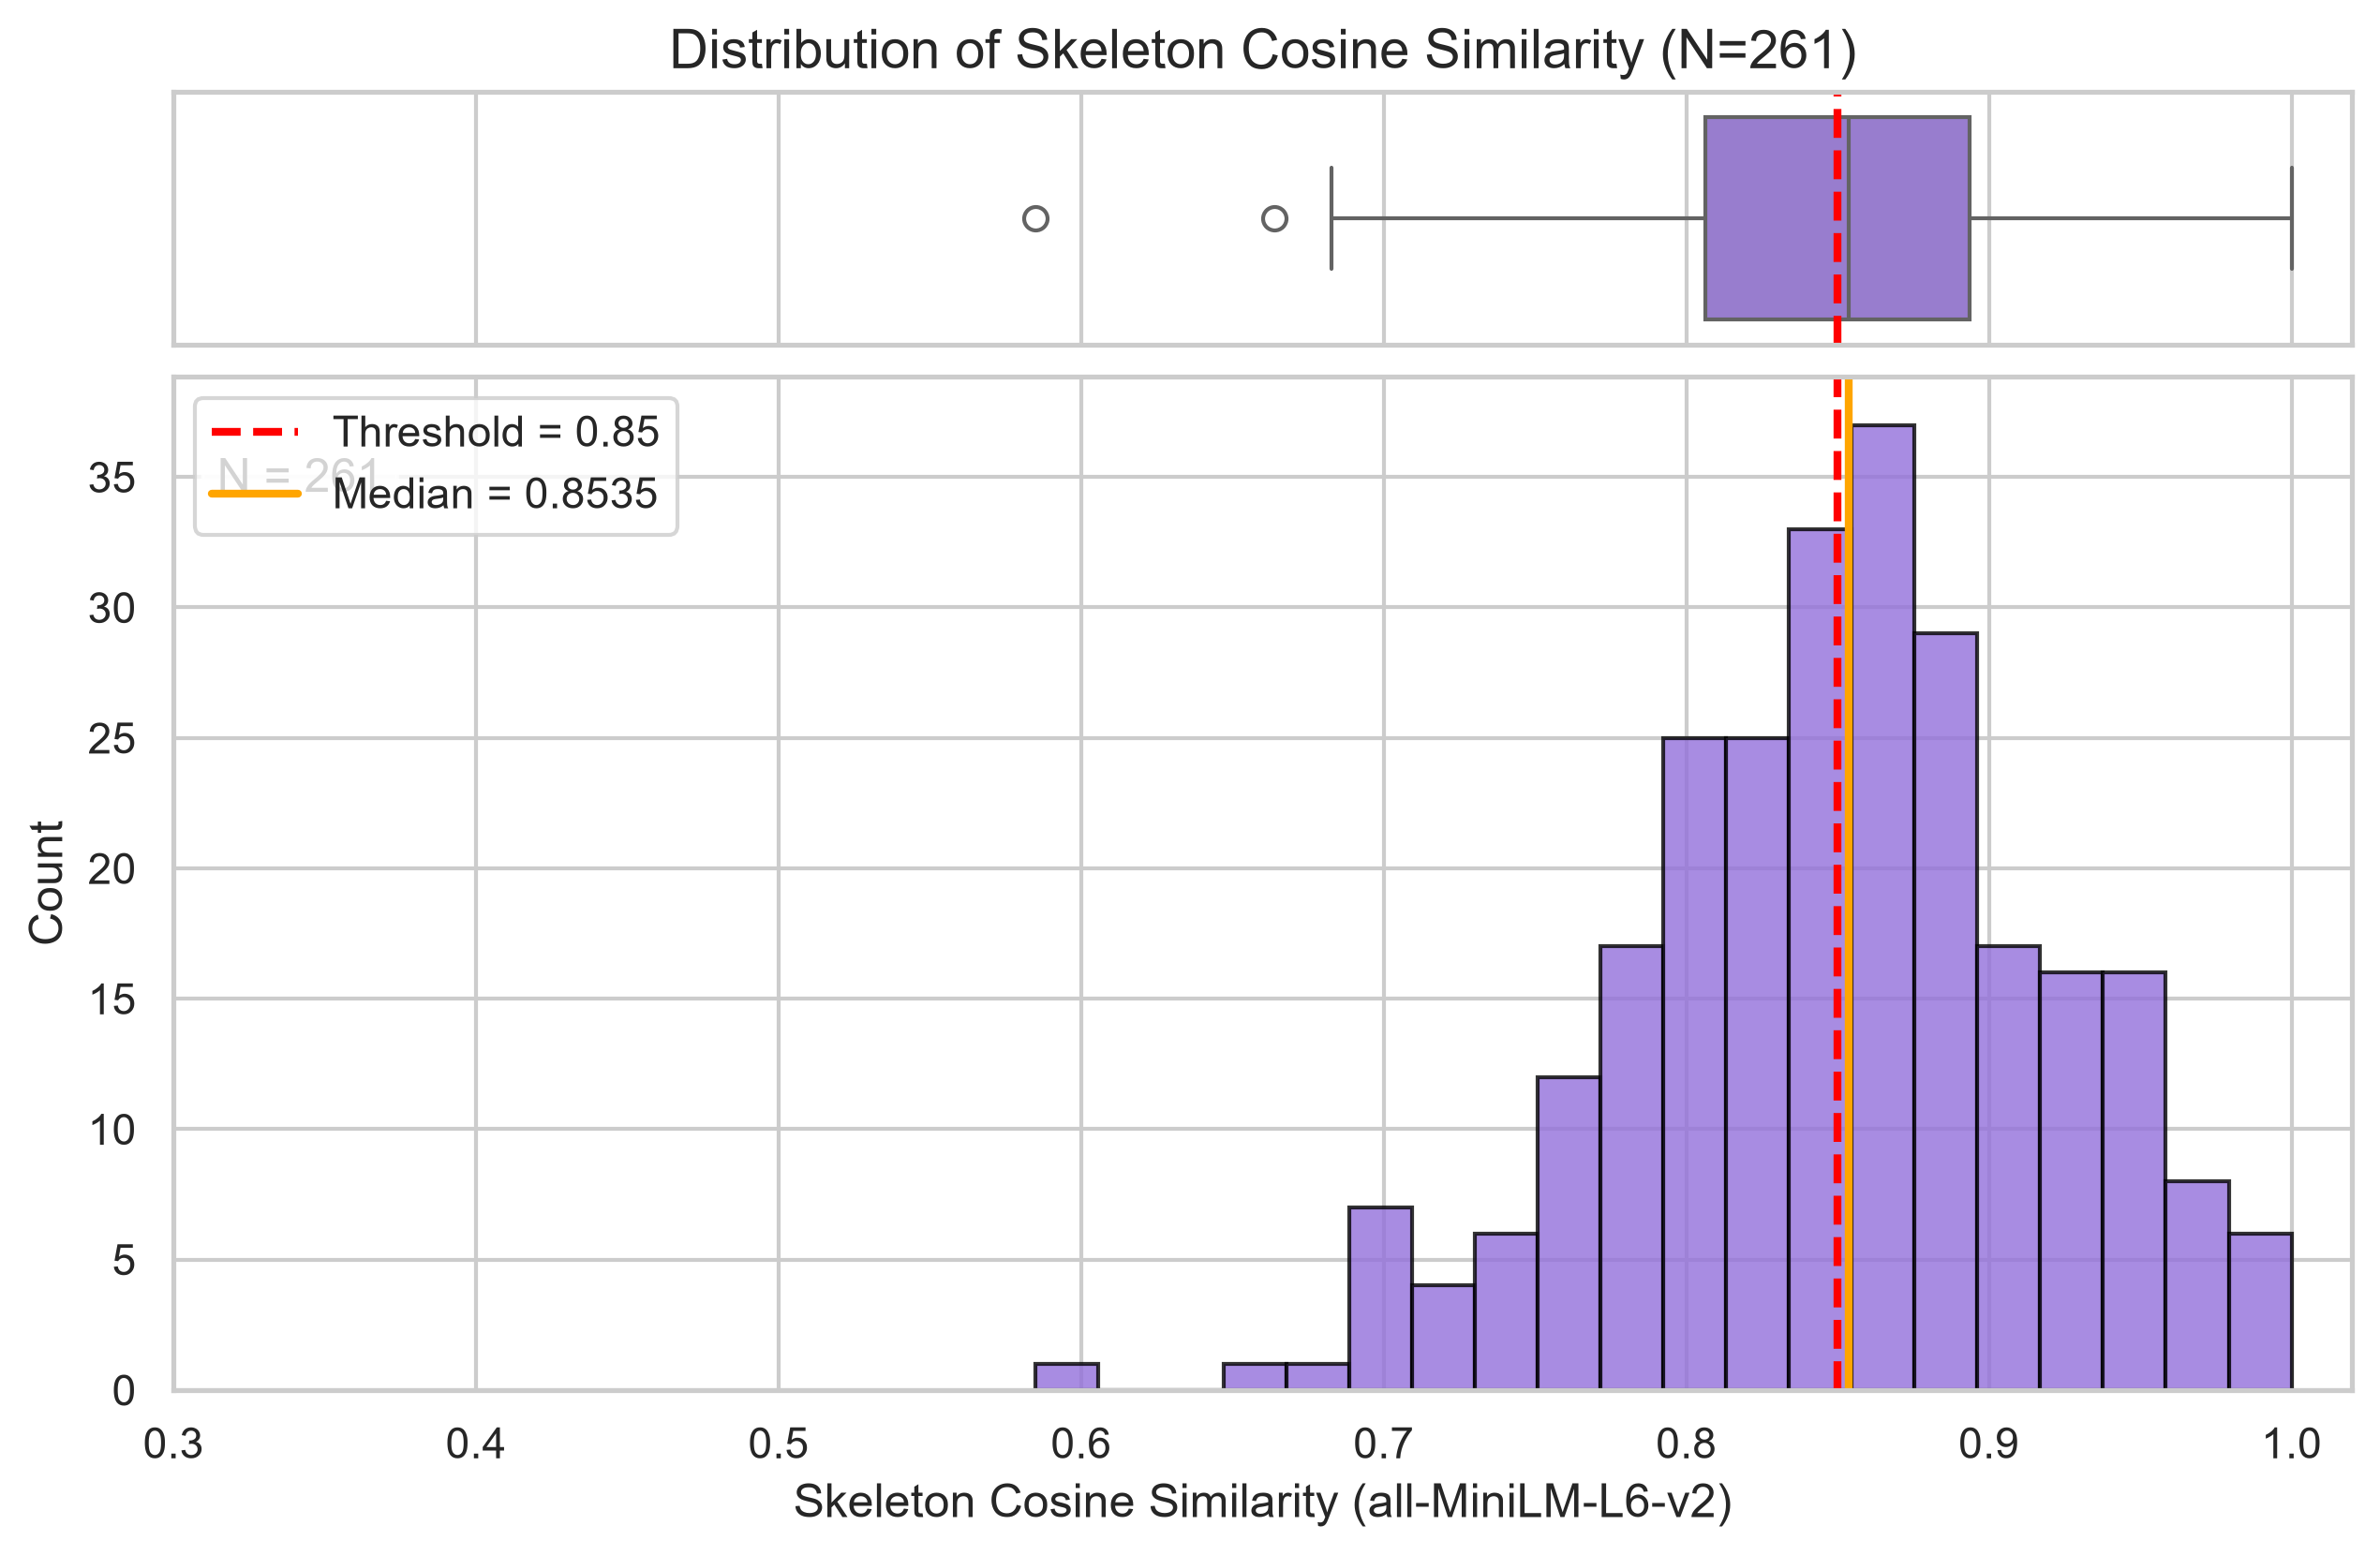
\includegraphics[width=0.85\linewidth]{figures/fig1_skeleton_distribution}
  \caption{Distribution of Skeleton Cosine Similarity scores for $N = 261$ generated
  scenarios. The red dashed line marks the acceptance threshold $\mu_0 = 0.85$;
  the orange line marks the sample median (0.853).}
  \label{fig:rq1-dist}
\end{figure}

Figure~\ref{fig:rq1-domain} breaks down these scores by the three business domains in our dataset. The variance across domains highlights why relying on a single project for evaluation can be misleading.

\begin{figure}[ht]
  \centering
  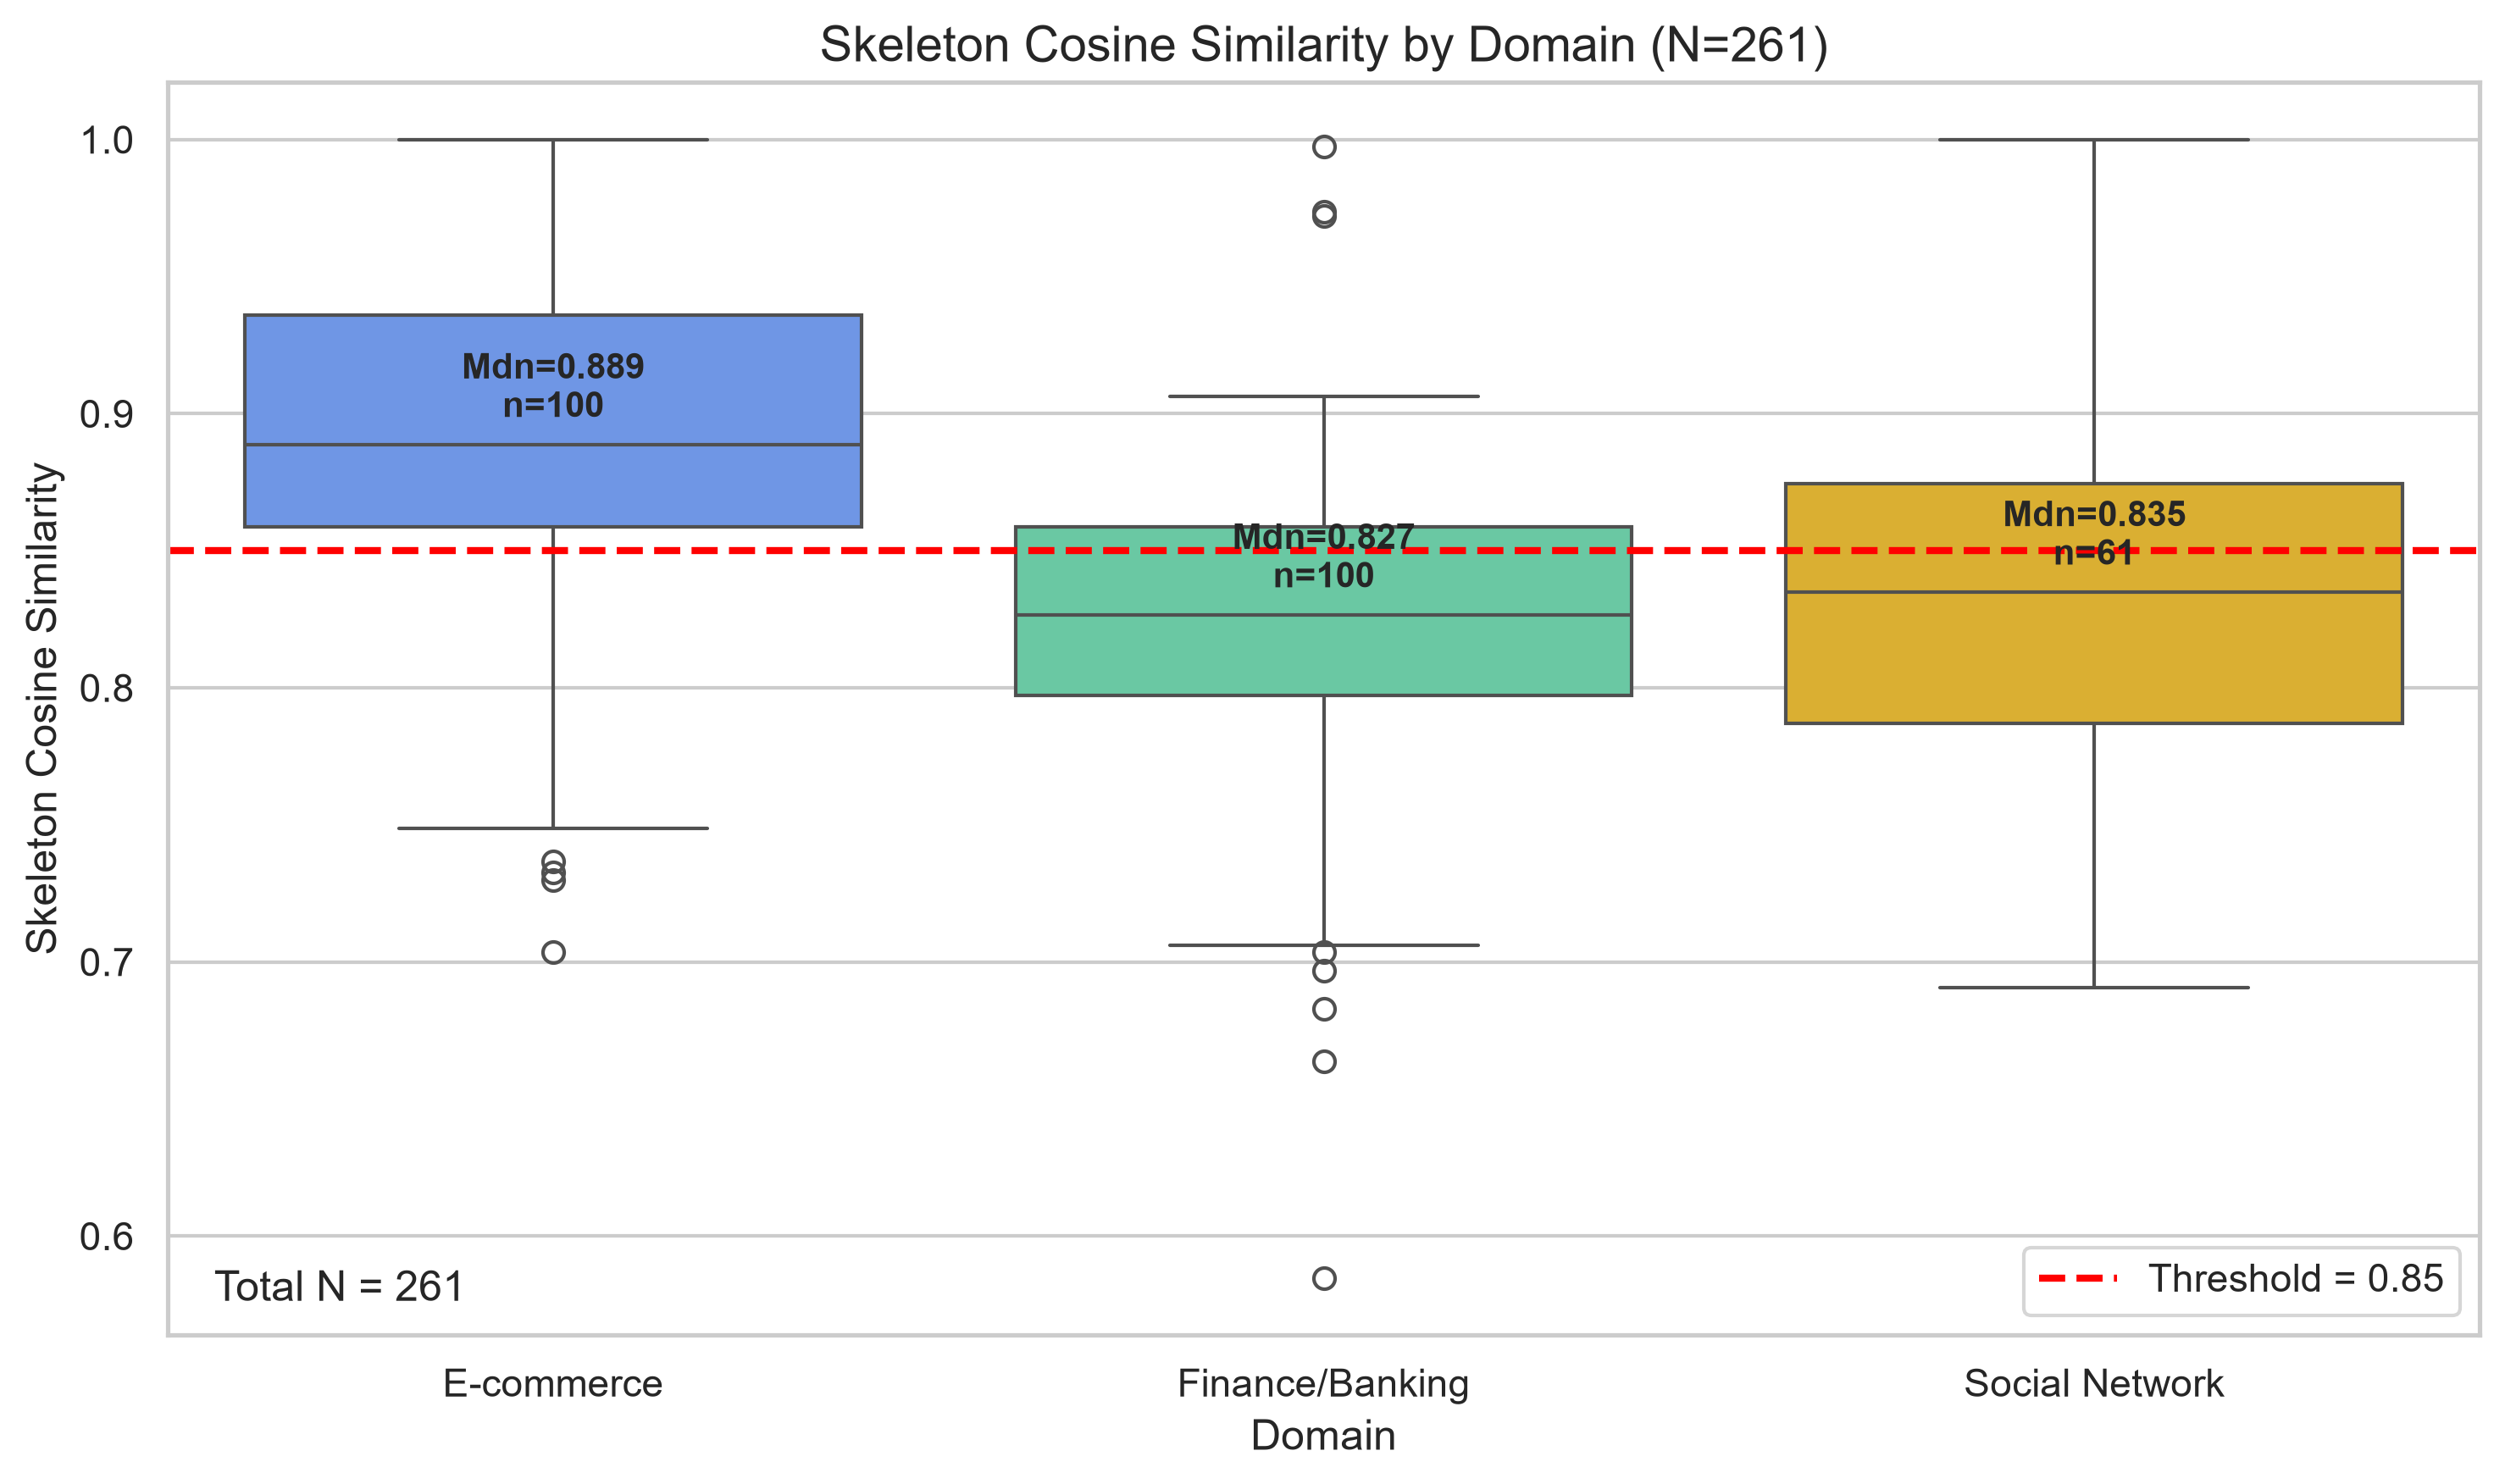
\includegraphics[width=0.85\linewidth]{figures/fig2_domain_comparison}
  \caption{Skeleton Cosine Similarity by Domain. E-commerce (Sylius) and Finance (Fineract) show high variance, while Social Network (Diaspora) remains more consistent.}
  \label{fig:rq1-domain}
\end{figure}

% ----------------------------------------------------------
\subsection{RQ2: Syntactic Correctness of Generated Gherkin (Executable Syntax Rate)}

\textbf{RQ2.} \textit{Does GPT-5.4-mini generate Gherkin scenarios that are executable
by the \texttt{behave} test runner at a rate above the acceptance threshold of 80\%?}

Table~\ref{tab:rq2-results} summarises the Executable Syntax Rate results.

\begin{table}[h]
\centering
\caption{Executable Syntax Rate results ($N = 261$).
The threshold $p_0 = 0.80$ is shown for reference.}
\label{tab:rq2-results}
\renewcommand{\arraystretch}{1.3}
\begin{tabular}{lc}
\toprule
\textbf{Statistic} & \textbf{Value} \\
\midrule
$N$ (total scenarios)              & 261        \\
Executable (behave --dry-run pass) & 261        \\
Non-executable (fail)              & 0          \\
\textbf{Executable Syntax Rate}    & \textbf{100.0\%} \\
Threshold $p_0$                    & 80.0\%     \\
\midrule
Exact Binomial $p$-value           & $< 0.001$  \\
95\% Clopper-Pearson CI            & [98.6\%, 100.0\%] \\
\bottomrule
\end{tabular}
\end{table}

All 261 generated scenarios (100\%) parsed and loaded without errors under
\texttt{behave --dry-run}.
The one-sided Exact Binomial test yields $p < 0.001$, far below $\alpha = 0.05$.
The 95\% Clopper-Pearson confidence interval for the true executable rate is
$[98.6\%, 100.0\%]$, which lies entirely above the threshold $p_0 = 0.80$.

\textbf{Decision:} We \textbf{reject} $H_0^{\text{RQ2}}$.
The evidence strongly supports the conclusion that GPT-5.4-mini generates syntactically
executable Gherkin at a rate significantly above the 80\% threshold.

Figure~\ref{fig:rq2-bar} visualizes this perfect pass rate.

\begin{figure}[ht]
  \centering
  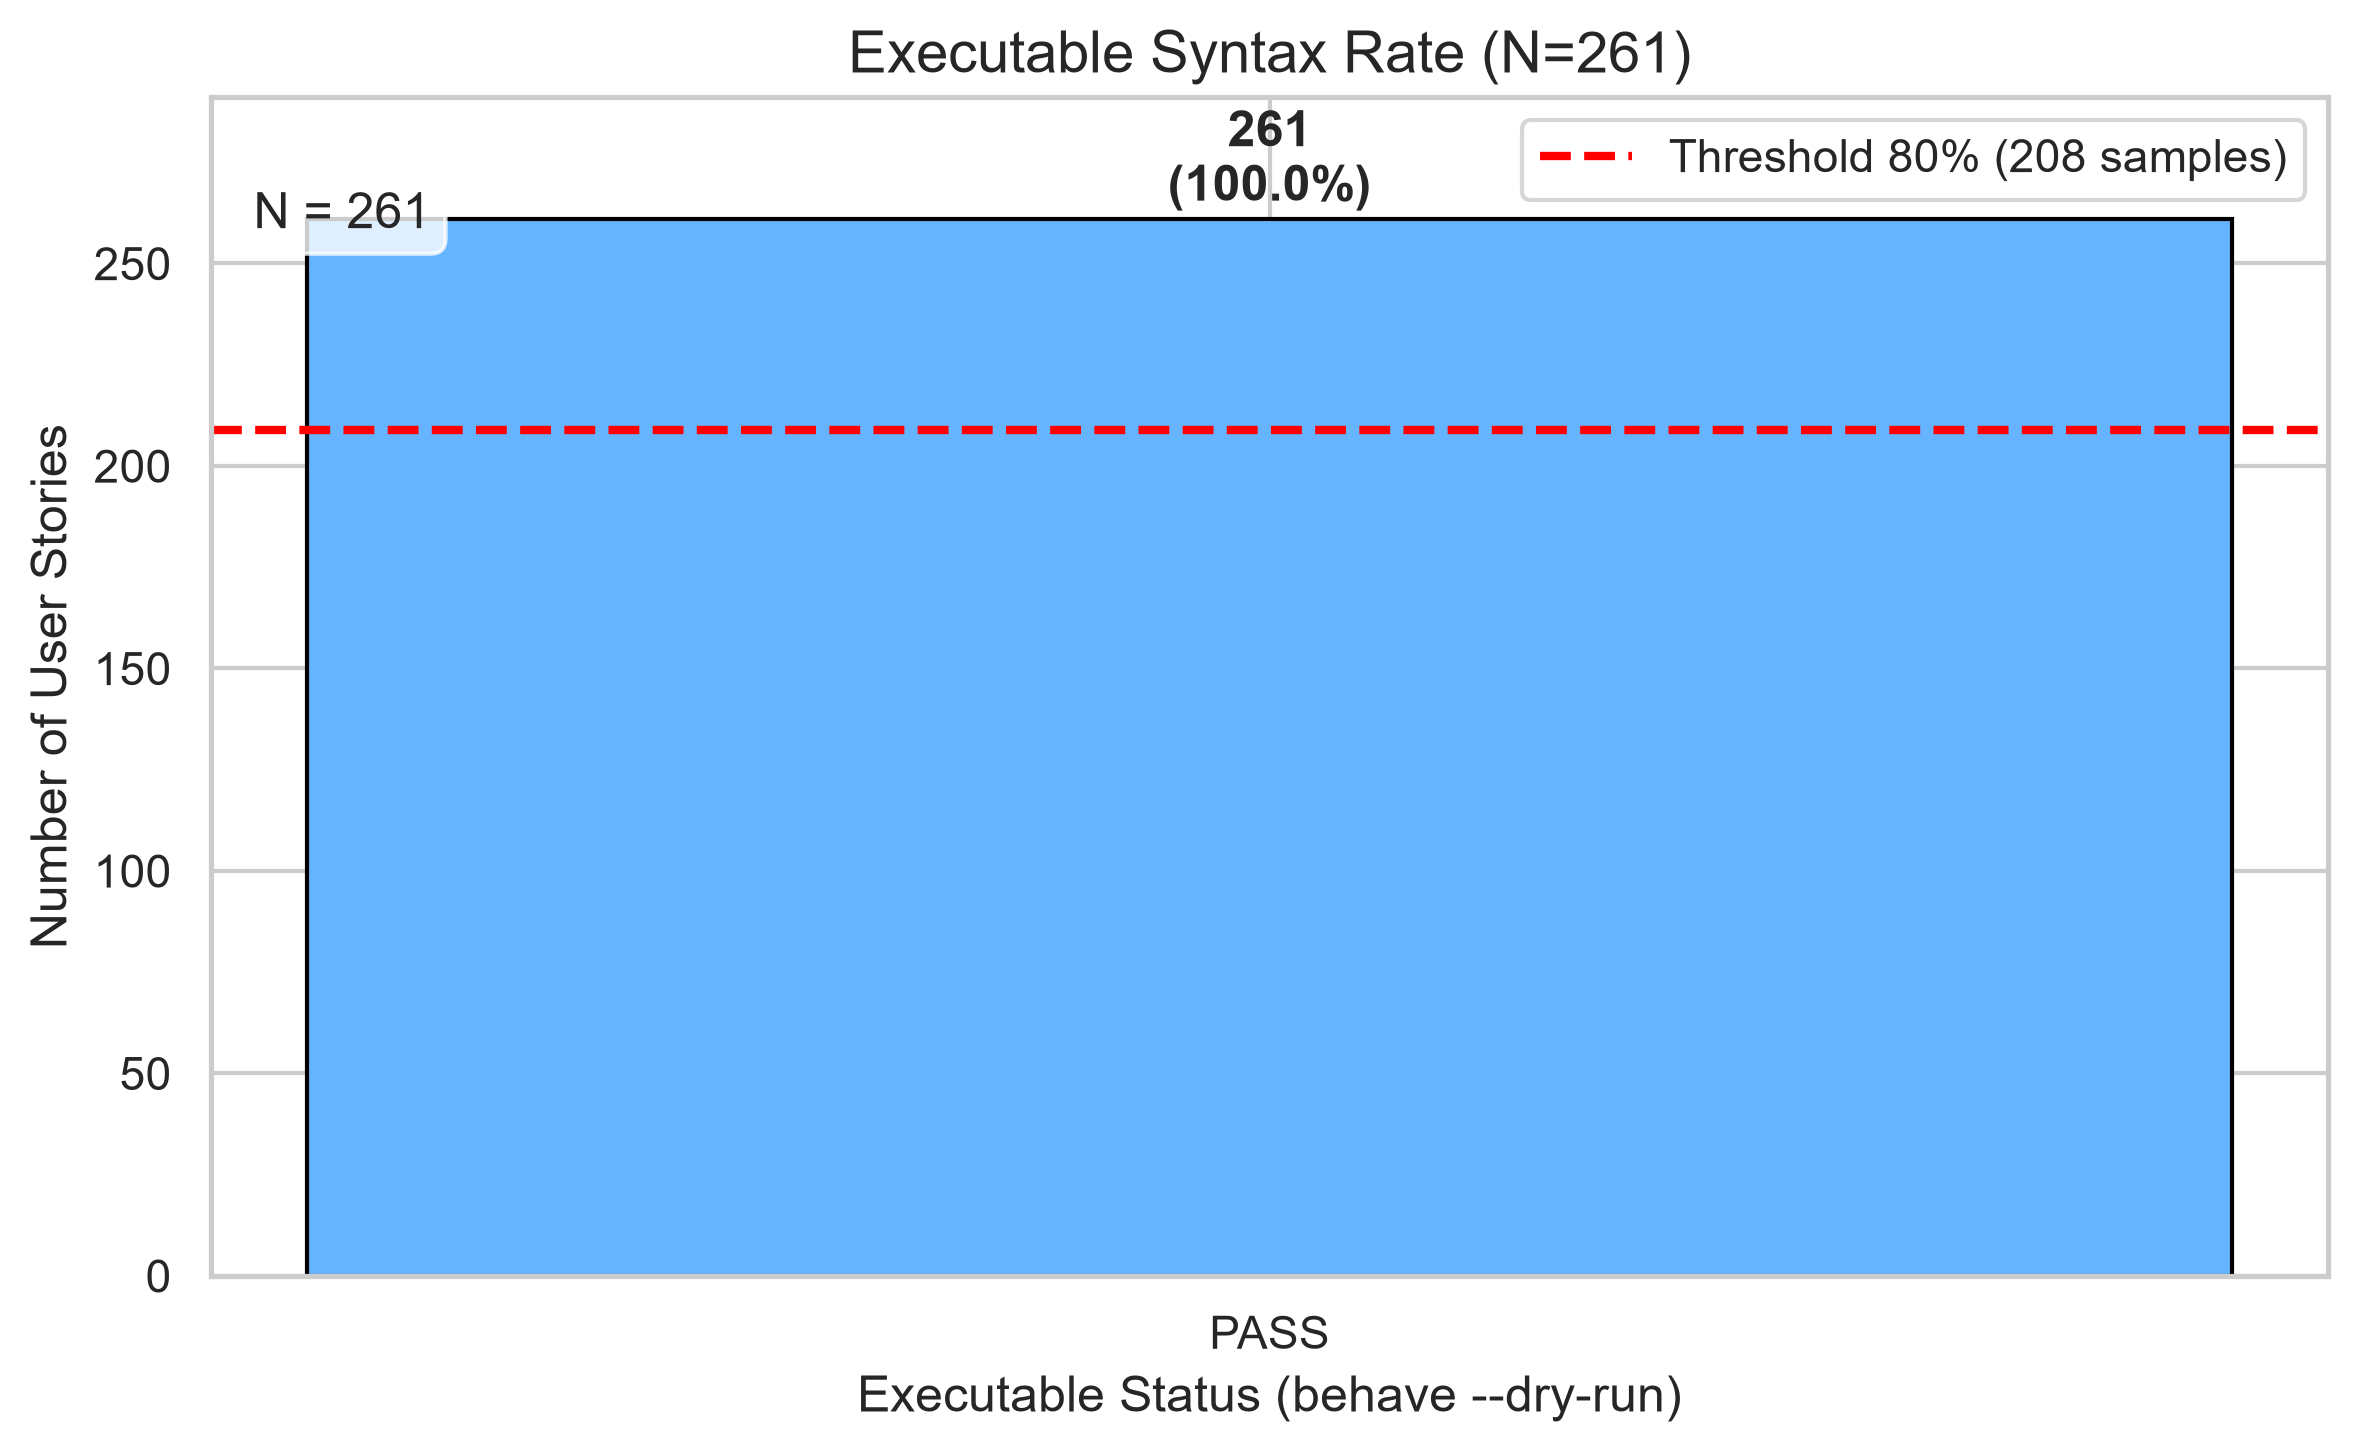
\includegraphics[width=0.75\linewidth]{figures/fig3_executable_rate}
  \caption{Executable Syntax Rate for $N=261$ generated scenarios. All scenarios successfully passed the \texttt{behave} parser without requiring manual syntax repair.}
  \label{fig:rq2-bar}
\end{figure}
